\documentclass[addpoints]{exam}
\usepackage[utf8]{inputenc}
\usepackage{amsmath}
\usepackage{tikz}
\usepackage{pgfplots}
\usetikzlibrary{datavisualization}
\usetikzlibrary{calc}
\usetikzlibrary{arrows}
\usetikzlibrary{decorations.pathreplacing,decorations.markings}
\usetikzlibrary{datavisualization.formats.functions}
\pgfplotsset{width=3cm,compat=1.4}
\usepackage{graphicx}%
\usepackage{mathtools}
\usepackage{dirtytalk}
\usepackage{relsize}
\graphicspath{ {images/} }
\DeclarePairedDelimiter{\ceil}{\lceil}{\rceil}
\usepackage{geometry}
\usepackage{draftwatermark}
\SetWatermarkFontSize{2cm}
\SetWatermarkText{সরল ছন্দিত স্পন্দন}
\usepackage[banglamainfont=Kalpurush, 
            banglattfont=Siyam Rupali
           ]{latexbangla}
        
\begin{document}
\begin{LARGE}
\begin{center}
সরল ছন্দিত স্পন্দন(Simple Harmonic Motion)
\end{center}
\end{LARGE}

1. \textbf{ PERIODIC MOTION}\\
When a body or a moving particle repeats its motion along a definite path after regular intervals of time, its
motion is said to be Periodic Motion and interval of time is called time period or harmonic motion period
(T). The path of periodic motion may be linear, circular, elliptical or any other curve. For example, rotaion of
earth about the sun.\\

2. \textbf{OSCILLATORY MOTION}\\
\say{To and Fro} type of motion is called an Oscillatory Motion. It need not be periodic and need not have fixed
extreme positions. For example, motion of pendulum of a wall clock.
The oscillatory motions in which energy is conserved are also periodic.
The force / torque (directed towards equilibrium point) acting in oscillatory motion is called restoring force /
torque.
Damped oscillations are those in which energy is consumed due to some resistive forces and hence total
mechanical energy decreases.\\

3. \textbf{SIMPLE HARMONIC MOTION}\\
If the restoring force/ torque acting on the body in oscillatory motion is directly proportional to the displacement of body/particle and is always directed towards equilibrium position then the motion is called simple
Harmonic Motion (SHM). It is the simplest (easy to analyse) form of oscillatory motion.\\
3.1 \textbf{TYPES OF SHM}\\
(a) Linear SHM : When a particle moves to and fro about an equilibrium point, along a straight line. A and B are
extreme positions. M is mean position. AM = MB = Amplitude.\\
(b) Angular SHM : When body/particle is free to rotate about a given axis executing angular oscillations.\\
3.2 \textbf{EQUATION OF SIMPLE HARMONIC MOTION (SHM) :}
The necessary and sufficient condition for SHM is
The necessary and sufficient condition for SHM is
$ F = – kx $
where k = positive constant for a SHM = Force constant
$ x $ = displacement from mean position.
\[m\dfrac{d^{2}x}{dt^{2}} = -kx\]


\textbf{বেগ বনাম সরণের লেখচিত্রঃ}\\
$ v=\omega \sqrt{A^{2}-x^{2}}\, \Rightarrow v^{2}=\omega^{2} (A^{2}-x^{2})\Rightarrow v^{2} + \omega^{2}x^{2} = \omega^{2}A^{2} \Rightarrow \dfrac{v^{2}}{\omega^{2}A^{2}} + \dfrac{x^{2}}{A^{2}} = 1$ যা একটি উপবৃত্তের সমীকরণ।

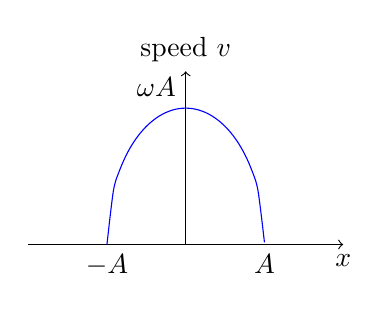
\begin{tikzpicture}
      \draw[->] (-2,0) -- (2,0);
      \draw[->] (0,0) -- (0,2.2) ;
      \draw (0,2.2)node[above] {speed $v$};
      \draw (0,2)node[left] {$\omega A$};
     \draw (2,0) node[below] {$x$};
     \draw (-1,0) node[below] {$-A$};
     \draw (1,0) node[below] {$A$};
      \draw[scale=0.5,domain=-2:2,smooth,variable=\x,blue] plot ({\x},{sqrt(3*(4-\x*\x))});
    \end{tikzpicture}


\end{document}